\chapter{Całki podwójne}

Zapis: $ \iint\limits_{D} f(x,y)\, dxdy $, gdzie zbiór $D$ i funkcja $f$ są odpowiednio regularne.

Definicja może być skonstruowana poprzez:
\begin{itemize}
    \item $n$ -- tą sumę całkową (sumę Riemanna) -- podobnie jak w AM1
    \item tzw. \underline{całki iterowane}
\end{itemize}
\bigskip

\begin{tw}{Całka w sensie Riemanna}
Przypadek podstawowy -- $D$ jest prostokątem
\[ D = [a,b] \times [c,d] = \{ (x,y): a \leq x \leq b, \ c \leq y \leq d \} \]

Dzielimy $D$ na $n$ prostokątów o bokach poziomych o długości $\Delta X$ i bokach pionowych o długości $\Delta y_i, \ i = 1,2,...,n$.
W każdym z prostokątów wybieramy dowolny punkt $P_i = (a_i, b_i)$.

Sumą Riemanna ($n$ -- tą sumę całkową) funkcji $f$ na $D$ jest
\[ S_n = \sum\limits_{n=1}^{n} \Delta x_i \cdot \Delta y_i \cdot f(a_i, b_i) \]
\end{tw}

\begin{center}
    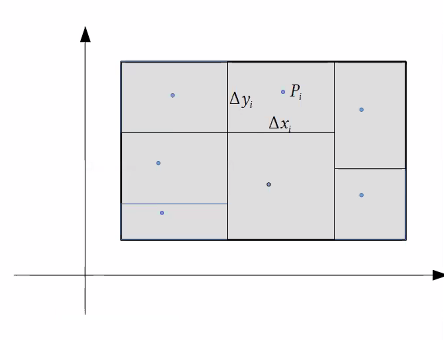
\includegraphics[scale=0.8]{img/prostokat1.png}
\end{center}

Jeżeli dla $ n \to \infty, \ \Delta x_i \to 0, \ \Delta y_i \to 0 $ \ granica \ $ \lim_{n \to \infty} S_n $ \ istnieje i \underline{nie zależy}
od wyboru prostokątów oraz punktów $P_i$ to nazywamy ją całką podwójną z $f$ na prostokącie $D$ i oznaczamy przez \ $ \iint\limits_D f(x,y) \, dxdy $.
\bigskip

\begin{tw}{Twierdzenie}

Gdy $f$ jest ciągła na prostokącie $D$ to całka podwójna z $f$ na $D$ istnieje.
\bigskip

Interpretacja geometryczna dla $ f \geq 0 $ na $D$: $S_n$ to suma objętości prostopadłościanów o krawędziach $ \Delta x_i, \ \Delta y_i $ oraz $ f(a_i, b_i) $.
Prostopadłościany te przybliżają bryłę o podstawie $D$, ścianach pionowych i ograniczonej z góry przez powierzchnię $f$.
\end{tw}


Granica $S_n$ daje objętość tej bryły.

\begin{center}
    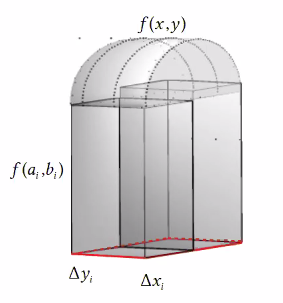
\includegraphics[scale=0.5]{img/prostowalec.png}
\end{center}

Dla $ D = [a,b] \times [c,d] $ są to całki postaci

\[ \int\limits_c^d dy \int\limits_{a}^{b} f(x,y) \, dx = \int\limits_{c}^{d} dy \left( \int\limits_{a}^{b} f(x,y) \, dx \right) \]
\begin{center}oraz \end{center}
\[ \int\limits_a^b dx \int\limits_{c}^{d} f(x,y) \, dy = \int\limits_{a}^{b} dx \left( \int\limits_{c}^{d} f(x,y) \, dy \right) \]

\begin{tw}{Twierdzenie}

Gdy $f$ jest ciągła na $D$ to
\[ \int\limits_{c}^{d} dy \int\limits_{a}^{b} f(x,y) \, dx = \int\limits_{a}^{b} dx \int\limits_{c}^{d} f(x,y) \, dy = \iint\limits_D f(x,y) \, dxdy \]

\end{tw}

\begin{przyklad}

\[ D = [0,1] \times [-1,1], \ f(x,y) = 2x + 3y^2 \]

\[ \int\limits_{0}^{1} dx \int\limits_{-1}^{1} (2x+3y^2) \, dy = \int\limits_{0}^{1} dx \left[ 2xy + y^3 \right]_{y = -1}^{y=1} 
= \int\limits_{0}^{1} dx (4x+2) = \left[ 2x^2 + 2x \right]_0^1 = 4 - 0 = 4 \]

\begin{center} W odwrotnej kolejności \end{center}
\[ \int\limits_{-1}^{1} dy \int\limits_{0}^{1} (2x+3y^2)\, dx = \int\limits_{-1}^{1} dy \left[ x^2 + 3y^2x \right]_{x=0}^{x=1} 
= \int\limits_{-1}^{1} dy (3y^2 + 1) = \left[ y^3 + y \right]_{-1}^{1} = 2- (-2) = 4 \]

Przypadek ogólny -- całki po tzw. \underline{obszarach normalnych}.

Są to zbiory postaci:
\[ D = \{ (x,y): a \leq x \leq b, \ d(x) \leq y \leq g(x) \} \quad \textrm{lub} \quad D = \{ (x,y): a \leq y \leq b, \ d(y) \leq x \leq g(y) \} \]

Ponadto funkcje $d$ i $g$ są ciągłe.
\end{przyklad}

\begin{tw}{Definicja}
Definicja całki podwójnej w sensie Riemanna jest analogiczna jak dla prostokąta.

\[ \int\limits_{a}^{b} dx \int\limits_{d(x)}^{g(x)} f(x,y)\, dy = \int\limits_{a}^{b} dx \left( \ \int\limits_{d(x)}^{g(x)} f(x,y)\, dy \right) \]
\begin{center} lub \end{center}
\[ \int\limits_{c}^{d} dy \int\limits_{d(x)}^{g(x)} f(x,y)\, dx = \int\limits_{a}^{b} dy \left( \ \int\limits_{d(x)}^{g(x)} f(x,y)\, dx \right) \]
\end{tw}

\begin{tw}{Twierdzenie}

Gdy $f$ jest ciągła na obszarze normalnym to całka podwójna $ \iint\limits_{D} f(x,y)\, dxdy $ istnieje i jest równa każdej z całek iterowanych. 

\end{tw}

\begin{przyklad}

$ f(x,y) = xy $

$D$ jest ograniczony krzywymi $ x=0, \ x=2, y=e^x $
\medskip

\begin{center}
    Rysunek obszaru:
    
    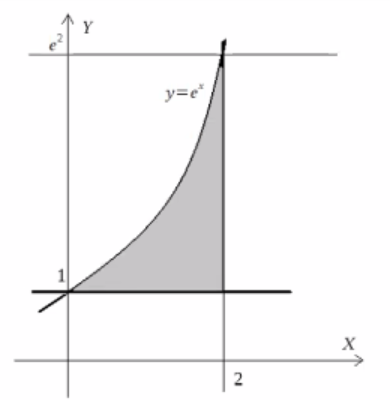
\includegraphics[scale=0.7]{img/krzywetrojkat.png}
\end{center}

Mamy \ $ D: 0 \leq x \leq 2, \ 1 \leq y \leq e^x $. Czyli całka jest równa
\[ \int\limits_{0}^{2} dx \int\limits_{1}^{e^x} xy \, dy = \int\limits_{0}^{2} dx \left[ \frac{xy^2}{2} \right]_{1}^{e^x} 
= \int\limits_{0}^{2} dx \left( \frac{xe^{2x}}{2} - \frac{x}{2} \right) = \frac{1}{2} \int\limits_{0}^{2} xe^{2x}\, dx - \frac{1}{2} \int\limits_{0}^{2} x\, dx \]

Ta druga całka wynosi 2.

Tą pierwszą liczymy przez części:
\[ \int xe^{2x} = \frac{1}{2} xe^{2x} - \int 1 \cdot \frac{1}{2} e^{2x} \, dx = \frac{1}{2} xe^{2x} - \frac{1}{4} e^{2x} + C \]
\[ \begin{vmatrix}
    f(x) = x & g'(x) = e^{2x} \\
    f'(x) = 1 & g(x) = \frac{1}{2}e^{2x} 
\end{vmatrix} \]

Zatem
\[ \int\limits_{0}^{2} xe^{2x} \, dx = e^4 - \frac{1}{4}e^4 + \frac{1}{4} = \frac{3}{4}e^4 + \frac{1}{4} \]

Całość:
\[ \iint\limits_D f(x,y) \, dxdy = \frac{1}{2} \left( \frac{3}{4}e^4 + \frac{1}{4} \right) - \frac{1}{2} \cdot 2 = \frac{3}{8}e^4 - \frac{7}{8} \]
\end{przyklad}

\begin{tw}{Własności całki podwójnej}
\begin{itemize}
    \item $ \iint\limits_D \left( f(x,y) \pm g(x,y) \right)\, dxdy = \iint\limits_D f(x,y)\, dxdy \pm \iint\limits_D g(x,y)\, dxdy $
    \item $ \iint\limits_D c \cdot f(x,y)\, dxdy = c \iint\limits_D f(x,y)\, dxdy $
    \item gdy \ $ D = D_1 \cup D_2 $ \ i \ $ D_1, D_2 $ \ są rozłączne to
    \[ \iint\limits_D f(x,y)\, dxdy = \iint\limits_{D_1} f(x,y)\, dxdy + \iint\limits_{D_2} f(x,y)\, dxdy \]
\end{itemize}
\end{tw}

\begin{tw}{Zmiana kolejności całkowania}
    \[ \iint\limits_D f(x,y)\, dxdy = \int\limits_{c}^{d} dy \int\limits_{d_1(y)}^{g_1(y)} f(x,y)\, dx \]
    będzie dawała jeden obszar i jedną całkę.
\end{tw}

Pytanie: jak mając obszar normalny względem $x$ zmienić go na obszar/obszary względem $y$?

Zmiana kolejności całkowania wymaga zmiany roli argumentu i wartości czyli np. mając funkcję brzegową $ y = f(x) $ trzeba wyliczyć ją względem $y$
czyli $x = g(y)$.

Związane jest to z wyznaczaniem \underline{funkcji odwrotnej}.

Stąd wniosek: zmiana kolejności całkowania jest związana z \textbf{odbiciem obszaru względem prostej $ y = x $}.

Funkcja/krzywa "prawa" staje się "górną", a "lewa" - "dolną".

Praktyczna uwaga: symetria względem prostej $y = x$ jest równoważna obrotowi względem $(0,0)$ w lewo o kąt $90^{\circ}$, a potem symetrii
względem osi pionowej.

W praktyce wystarczy sam obrót by zobaczyć funkcje górne i dolne.

\begin{przykladbig}
Zapisać, jako całkę iterowaną, $ \iint\limits_D f(x,y)\, dxdy $, gdzie $D$ jest obszarem na rysunku poniżej.

Następnie zmienić kolejność całkowania.

\begin{center}
    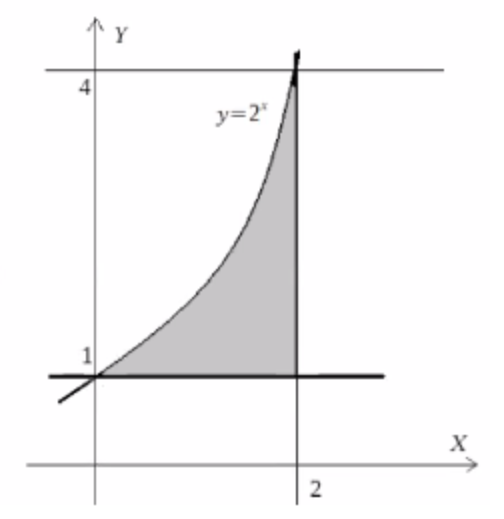
\includegraphics[scale=0.5]{img/2x.png}
\end{center}

Widać, że funkcją dolną jest funkcja stała $y=1$, a górną $y = 2^x$. Zmienność $x$ można odczytać poprzez rzut obszaru na oś $X$.

Zatem
\[ D: \ 0 \leq x \leq 2, \quad 1 \leq y \leq 2^x \]
To daje całkę 
\[ \int\limits_{0}^{2} dx \int\limits_{1}^{2^x} f(x,y)\, dy \]

\textbf{Ważna uwaga}

Jeżeli zarówno $x$ jak i $y$ są ograniczone przez liczby to obszar jest prostokątem lub sumą prostokątów. Zatem każdy zbiór,
który nie jest prostokątem/sumą prostokątów będzie zawierał \textbf{zależność jednej zmiennej od drugiej}.

\begin{blad}{Popularny błąd}
Obie zmienne między liczbami dla obszarów innych niż prostkąty

Na przykład dla naszego obszaru
\[ D : \ 0 \leq x \leq 2, \quad \textcolor{red}{1 \leq y \leq 4} \]
GAME OVER... To jest opis prostokąta
\end{blad}

Teraz zmiana kolejności całkowania.

Funkcją górną staje się krzywa prawa (prosta pionowa), a dolną -- lewa $(y=2^x)$.

Widać to po obrocie rysunku względem (0,0) w lewo o kąt $90^{\circ}$.

\begin{center}
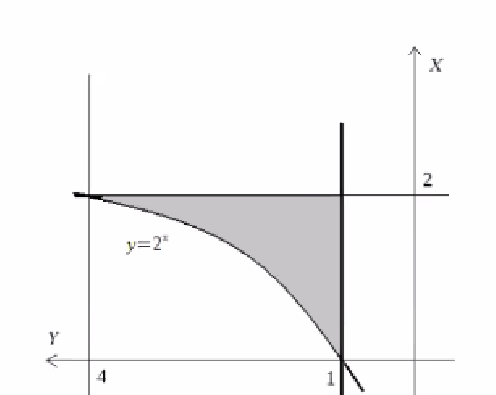
\includegraphics[scale=0.45]{img/2xzlewej.png}
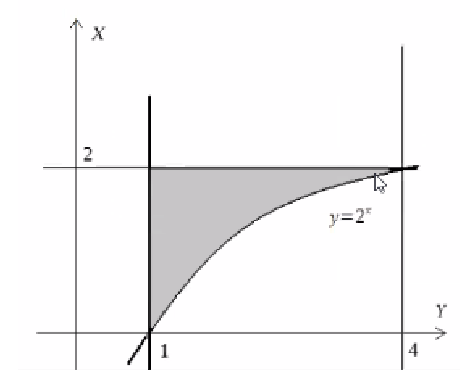
\includegraphics[scale=0.45]{img/2xzprawej.png}
\end{center}

Zatem dostaniemy
\[ y = 2^x \ \Leftrightarrow \ x = \log_2 y \ \textrm{-- funkcja dolna} \]
\[ x = 2 \ \textrm{-- funkcja górna} \]

Warunki opisujące $D: \ 1 \leq y \leq 4, \quad \log_2 y \leq x \leq 2$

Całka: $ \int\limits_{1}^{4} dy \int\limits_{\log_2 y}^{2} f(x,y)\, dx $
\end{przykladbig}

Praktyczna uwaga.

Opłaca się zmieniać kolejność całkowania, gdy w podstawowym zapisie trzeba dzielić obszar na kilka fragmentów, a po zmianie dostajemy jeden
obszar (między jedną funkcją górną i jedną dolną).
\begin{przyklad}
    Na przykład poniższy w postaci $ D = \{(x,y): \ a \leq x \leq b, \ d(x) \leq y \leq g(x) \} $
    
    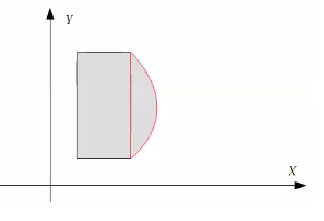
\includegraphics[scale=0.65]{img/obszar1.png}

    trzeba rozbić na sumę 2 obszarów i będą 2 całki

    Po zmianie kolejności całkowania mamy obszar w postaci

    $ D = \{(x,y): \ c \leq y \leq d, \ d_1(y) \leq x \leq g_1(y) \} $

    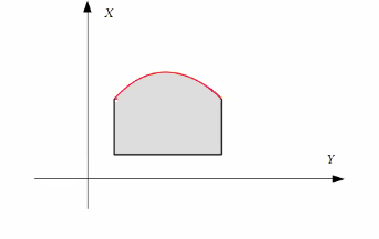
\includegraphics[scale=0.6]{img/obszar2.png}

    Będzie to całka po tylko jednym obszarze.
\end{przyklad}

\subsection{Zmiana zmiennych w całce podwójnej}

Chodzi o metodę podstawienia

Wyprowadzamy wzory

$ x = x(s,t) $

$ y = y(s,t) $

Zakładamy, że są to różniczkowalne funkcje zmiennych $s$ i $t$.

$s$, $t$ -- nowe współrzędne,

$x$, $y$ -- stare współrzędne.

Definiujemy wyznacznik

\[ J = J(s,t) = \begin{vmatrix}
    \frac{dx}{ds} & \frac{dx}{dt} \\
    \frac{dy}{ds} & \frac{dy}{dt}
\end{vmatrix} \textrm{\quad -- \underline{jakobian} przekształcenia} \]

$A$ - obraz $D$ w nowych współrzędnych tzn. \ $ (x,y) \in D \ \Leftrightarrow \ (s,t) \in A $.

Wtedy mamy wzór
\[ \iint\limits_D f(x,y) \, dxdy = \iint\limits_A f(x(s,t), y(s,t)) \cdot |J|\, dsdt \]

Jest to metoda podstawienia w całce podwójnej.


\subsection{Współrzędne biegunowe}

Jest to szczególny przypadek podstawienia.

Współrzędne biegunowe \underline{centralne} -- mają środek w (0,0).

Jest to odpowiednik postaci trygonometrycznej dla liczb zespolonych:
\begin{itemize}
    \item $r$ -- odległość punktu $(x,y)$ od środka (0,0)
    \item $\varphi$ -- kąt między dodatnią częścią osi X oraz półprostą łączącą środek z $(x,y)$
\end{itemize}

\begin{tw}{Formalne wzory}
\[ x = r \cos \varphi \]
\[ y = r \sin \varphi \]
\[ J = r \geq 0 \]
\[ 0 \leq \varphi < 2 \pi \quad \textrm{lub} \quad -\pi < \varphi \leq \pi \]

Obliczenie jakobianu:
\[ J = J(r, \varphi) = \begin{vmatrix}
    \cos \varphi & -r \sin \varphi \\
    \sin \varphi & r \cos \varphi
\end{vmatrix} = r \cos^2 \varphi - (- r \sin^2 \varphi) = r(\cos^2 \varphi + \sin^2 \varphi) = r \geq 0 \]

\end{tw}

Zatem $ |J| = r $.

Stosujemy gdy jest dużo wyrażeń typu $x^2 + y^2 = R^2 $.

Obraz zbioru $D$ we współrzędnych biegunowych zwykle ma postać
\[ A = A(r, \varphi) = \{ (r, \varphi): \ a \leq \varphi \leq \beta, \ d(\alpha) \leq r \leq g(\alpha) \} \]

Warunek \ $ a \leq \varphi \leq \beta $ \ zwykle można wywnioskować z rysunku.

Warunek \ $ d(\alpha) \leq r \leq g(\alpha) $ \ zwykle wymaga obliczeń, bo najczęściej promień zależy od kąta.

\textbf{Praktyczna obserwacja:} promień nie zależy od kąta, gdy obszar jest
\begin{itemize}
    \item kołem lub wycinkiem kątowym o wierzchołku w (0,0)
    \item pierścieniem kołowym o środku w (0,0)
    \item sumą lub przekrojem powyższych zbiorów
\end{itemize}

\textbf{Inny środek niż w (0,0) powoduje, że promień zależy od kąta}

\subsection{Współrzędne biegunowe przesunięte -- o środku w $(x_0, y_0)$}
\begin{itemize}
    \item r -- odległość punktu $(x,y)$ od środka $(x_0, y_0)$,
    \item $\varphi$ -- kąt między półprostą $ y = y_0, \ x \geq x_0 $ \ oraz półprostą łączącą środek z $(x,y)$.
\end{itemize}

\begin{center}
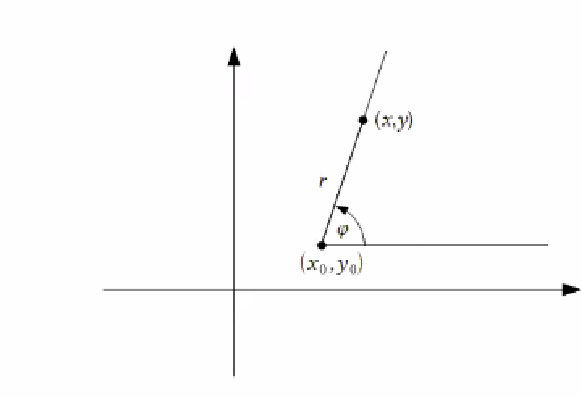
\includegraphics[scale=0.5]{img/katbiegun.png}
\end{center}

\begin{tw}{Formalne wzory}
\[ x = x_0 + r \cos \varphi \]
\[ y = y_0 + r \sin \varphi \]
\[ J = r \geq 0 \]
\[ 0 \leq \varphi < 2 \pi \quad \textrm{lub} \quad -\pi < \varphi \leq \pi \]
\end{tw}

Stosujemy, gdy jest dużo wyrażeń typu \ $ (x - x_0)^2 + (y - y_0)^2 = R^2 $

Postać obrazu zbioru $D$ oraz praktyczne uwagi są analogiczne do przypadku centralnego, jednak wszystko odnosimy do środka $(x_0, y_0)$, a nie (0,0).

\begin{przykladbig}
    \[ \iint\limits_D xy^2, \quad D: \ x^2 + y^2 \leq 4, \quad x \geq 0 \]

    Rysunek obszaru
    
    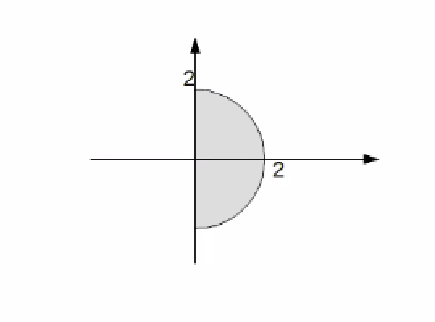
\includegraphics[scale=0.4]{img/polokrag.png}

    Wyznaczenie $r$ i $\varphi$

    a) Z rysunku $ -\frac{\pi}{2} \leq \varphi \leq \frac{\pi}{2}, \ 0 \leq r \leq 2$

    b) Z obliczeń

    $ r^2 \leq 4 $ \ oraz \ $ r \cos \varphi \geq 0 \ \Leftrightarrow \ 0 \leq r \leq 2 $ \ oraz \ $ \cos \varphi \geq 0 $.

    Dla cosinusa wygodniej brać \ $ -\pi < \varphi \leq \pi $ \ zamiast \ $ 0 \leq \varphi < 2\pi $.

    Wtedy

    $ \cos \varphi \geq 0 \ \Leftrightarrow \ -\frac{\pi}{2} \leq \varphi \leq \frac{\pi}{2} $

    \[ \iint\limits_D xy^2 = \int\limits_{-\frac{\pi}{2}}^{\frac{\pi}{2}} d\varphi \int\limits_{0}^{2} r \, dr \cdot r \cos \varphi \cdot (r \sin \varphi)^2 
    = \int\limits_{-\frac{\pi}{2}}^{\frac{\pi}{2}} d \varphi \, \cos \varphi \sin^2 \varphi \int\limits_{0}^{2} r^4 \, dr \]
    \[ = \frac{32}{5} \int\limits_{-\frac{\pi}{2}}^{\frac{\pi}{2}} d \varphi \, \cos \varphi \sin^2 \varphi = [t = \sin \varphi] \ \frac{32}{5} \int\limits_{-1}^{1} t^2 \, dt = \frac{64}{15} \]
\end{przykladbig}

\begin{przykladbig}
    \[ \iint\limits_D (x^2 + y^2) \, dxdy, \quad D: \ x^2 + y^2 + 2y \leq 0 \]

    $D$ -- koło o środku w (0, -1) i promieniu 1: $ x^2 (y+1)^2 \leq 1 $.

    Zastosujemy 2 metody. \bigskip

    a) Współrzędne centralne

    Z rysunku widać, że \ $ \pi \leq \varphi < 2\pi $:

    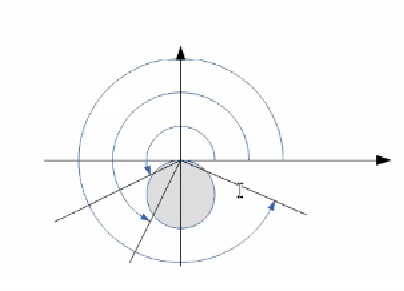
\includegraphics[scale=0.5]{img/kolkakat.png}

    Promień zależy od kąta bo nasze koło nie ma środka w (0,0).

    Po wstawieniu warunku na $D$:
    \[ r^2 + 2r \sin \varphi \leq 0 \ \Leftrightarrow \ r \leq -2 \sin \varphi \quad (\textrm{bo} \ r \geq 0) \ \textrm{czyli} \ 0 \leq r \leq -2 \sin \varphi \]

    Jeżeli chcemy potwierdzić zasięg kąta obliczeniami to pojawia się pytanie: skąd wziąć warunek na kąt? \bigskip

    \textbf{Zawsze jest dodatkowy (pośredni) warunek: funkcja dolna $ \leq $ funkcja górna}

    U nas to daje
    \[ 0 \leq -2 \sin \varphi \quad \textrm{czyli} \quad \sin \varphi \leq 0 \quad \textrm{a stąd} \quad \pi \leq \varphi < 2 \pi \]
    \[ \int\limits_{\pi}^{2\pi} d \varphi \int\limits_{0}^{-2\sin\varphi} rdr \cdot r^2 = \int\limits_{\pi}^{2\pi} d \varphi 4 \sin^4 \varphi = 
    ...[\text{dość długa całka}]... = \]
    \[ 4 \left[ \frac{3}{8}\varphi - \frac{1}{4}\sin(2\varphi) + \frac{1}{32}\sin(4\varphi) \right]_{\pi}^{2\pi} = \frac{3}{2}\pi \]

    \bigskip
    b) Przesunięte współrzędne: środek to (0, -1).

    Wtedy
    \[ x = r \cos \varphi, \quad y = -1 + r \sin \varphi, \quad x^2 + (y+1)^2 = r^2 \]

    $r$ -- odległość od (0, -1),
    $\varphi $ -- kąt względem półprostej \ $ y = -1, \ x \geq 0 $.

    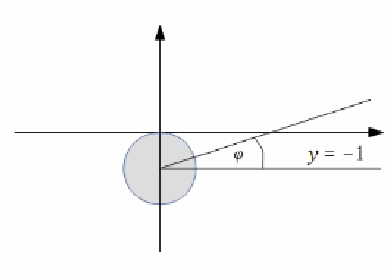
\includegraphics[scale=0.6]{img/okragikat.png}

    To daje \ $ 0 \leq \varphi < 2\pi, \ 0 \leq r \leq 1 $.

    Dostajemy
    \[ \int\limits_{0}^{2\pi} d \varphi \int\limits_{0}^{1} r \, dr \cdot (r^2 \cos^2 \varphi + (-1 + r \sin \varphi)^2) 
    = \int\limits_{0}^{2\pi} d \varphi \int\limits_{0}^{1} r \, dr \cdot (r^2 - 2r \sin \varphi + 1) \]
    \[ = \int\limits_{0}^{2\pi} d \varphi \left[ \frac{1}{4} r^2 - 2 \frac{r^3}{3} \sin \varphi + \frac{r^2}{2} \right]_0^1
    = \int\limits_{0}^{2\pi} d \varphi \left( \frac{3}{4} - \frac{2}{3} \sin \varphi \right) = \frac{3}{2} \pi \]

    Ten sam wynik co poprzednio ale całka łatwiejsza.
\end{przykladbig}

\textbf{Uwaga}

Szczególny przypadek występuje, gdy w wewnętrznej całce (po $r$) ani funkcja ani granice całkowania nie zależą od kąta $\varphi$.
Wtedy jest ona stała względem $\varphi$ i można ją wyciągnąć na zewnątrz.

Daje to wzór typu

\begin{center}
"długość przedziału dla kąta $\cdot$ całka wewnętrzna"
\end{center}

i pozwala uprościć rachunki.

\begin{przyklad}
    \[ \int\limits_{\frac{\pi}{3}}^{\pi} \, d\varphi \int\limits_{1}^{2} r\, dr = \frac{2}{3} \pi \int\limits_{1}^{2} r\, dr = \frac{2}{3}\pi \cdot \frac{3}{2} = \pi \]
\end{przyklad}

Pole $D$: $ |D| = \iint\limits_D 1 \, dxdy $

Gdy $D$ jest dany warunkami
\[ D : a \leq x \leq b, \quad d(x) \leq y \leq g(x) \]
to dostajemy
\[ \iint\limits_D \, dxdy = \int\limits_{a}^{b} dx \int\limits_{d(x)}^{g(x)} dy = \int\limits_{a}^{b} dx (g(x) - d(x)) \quad \text{-- wzór z AM1} \]
Zatem wzór \ $ |D| = \iint\limits_D 1 \, dxdy $ \ daje coś nowego, gdy chcemy wprowadzić nowe zmienne, np. przejść na współrzędne biegunowe.

\begin{przykladbig}
    \textit{Wersja zadania egzaminacyjnego z 1997 roku} \medskip

    Na poniższym rysunku zaznaczony jest obszar pomiędzy dwoma okręgami stycznymi i linią prostą.
    Przy pomocy całki podwójnej obliczyć jego pole.

    \begin{center}
        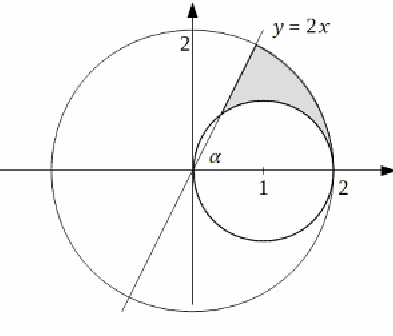
\includegraphics[scale=0.5]{img/egzamokrag.png}
    \end{center}

    Okrąg zewnętrzny ma równanie \ $ x^2 + y^2 = 4 $

    Okrąg wewnętrzny ma równanie \ $ (x-1)^2 + y^2 = 1 \ \Leftrightarrow \ x^2 + y^2 = 2x $

    Dowolny punkt $(x,y)$ z danego obszaru spełnia zatem następujące warunki:
    \begin{itemize}
        \item leży po zewnętrznej stronie okręgu wewnętrznego, a stąd \ $ x^2 + y^2 \geq 2x $
        \item leży po wewnętrznej stronie okręgu zewnętrznego, a stąd \ $ x^2 + y^2 \leq 4 $
        \item leży pomiędzy osią $X$ oraz prostą \ $ y = 2x $ \ a stąd \ $ 0 \leq y \leq 2x $
    \end{itemize}

    We współrzędnych kartezjańskich nasz obszar jest zatem zbiorem
    \[ D = \{ (x,y): 2x \leq x^2 + y^2 \leq 4, \ \ 0 \leq y \leq 2x \} \]

    Wprowadzamy współrzędne biegunowe $r$ i $\varphi$.
    
    Pierwszy z warunków na $D$ prowadzi do nierówności \ $ 2r \cos \varphi \leq r^2 \leq 4 $

    Stąd \ $ 2 \cos \varphi \leq r \ \leq 2 $

    Ten warunek zachodzi dla wszystkich wartości kąta $\varphi$, bo zawsze \ $ 2\cos \varphi \leq 2 $.

    Drugi warunek oznacza, że \ $ 0 \leq r \sin \varphi \leq 2r \cos \varphi $.

    Stąd wynika, że \ $ \sin \varphi \geq 0 $ \ oraz \ $ \cos \varphi \geq 0 $, \ a więc na pewno \ $ \varphi \in \left[ -\frac{\pi}{2}, \frac{\pi}{2} \right] $,
    co widać od razu z rysunku.

    Ponieważ \ $ \cos \varphi \geq 0 $, \ powyższą podwójną nierówność można podzielić przez \ $ r \cos \varphi $ tak, by sprowadzić ją do funkcji $\tan$:
    \[ 0 \leq \frac{r \sin \varphi}{r \cos \varphi} \leq 2 \ \Leftrightarrow \ 0 \leq \tan \varphi \leq 2 \]

    Ponieważ \ $ \varphi \in \left[ -\frac{\pi}{2}, \frac{\pi}{2} \right] $, \ oznacza to, że \ $ 0 \leq \varphi \leq \arctan 2 $

    To jest ostateczny warunek na kąt.

    Można go także wywnioskować bezpośrednio z rysunku.

    Zaznaczony na rysunku kąt $\alpha$ jest kątem nachylenia prostej $y = 2x$ do osi $X$ zatem ma miarę $\arctan 2$.
    Jest to największa możliwa wartość $\varphi$.

    Najmniejsza występuje dla punktu (2,0) i wynosi 0.

    Ostatecznie, $D$ jest obrazem zbioru
    \[ A = \{ (r, \varphi): 0 \leq \varphi \leq \alpha = \arctan 2, \ \ 2 \cos \varphi \leq r \leq 2 \} \]

    To daje
    \[ |D| = \iint\limits_D 1\, dxdy = \int\limits_{0}^{a} d \varphi \int\limits_{2 \cos \varphi}^{2} r\, dr \cdot 1 =
    \int\limits_{0}^{\alpha} d\varphi \left[ \frac{r^2}{2} \right]_{2 \cos \varphi}^{2} = \int\limits_{0}^{\alpha} d\varphi (2 - 2\cos^2 \varphi) = \]
    \[ 2 \int\limits_{0}^{\alpha} (1 - \cos^2 \varphi) \, d\varphi = 2 \int\limits_{0}^{\alpha} \sin^2 \varphi \, d \varphi =
    2 \left[ \frac{1}{2} \varphi - \frac{1}{4} \sin (2\varphi) \right]_{0}^{\alpha} = \alpha  - \frac{1}{2} \sin (2\alpha) = \]
    \[ \arctan 2 - \frac{1}{2} \sin(2 \arctan 2) \]
    
    Wynik ten można nieco uprościć wiedząc, że \ $\tan \alpha = 2$ i korzystając z tożsamości $ \sin (2\alpha) = \frac{2 \tan \alpha}{1 + \tan^2 \alpha} $,
    co daje $ \sin (2\alpha) = \frac{4}{5} $. \medskip

    Ostatecznie
    \[ |D| = \arctan 2 - \frac{2}{5} \]
\end{przykladbig}

Zadanie dodatkowe: obliczyć to pole korzystając bezpośrednio z geometrii, analizując pola odpowiednich wycinków kołowych oraz trójkątów.

\begin{tw}{Definicja}
    Wartość średnia funkcji na zbiorze $D$:
    \[ f_{\text{śr}} = \frac{\displaystyle\iint\limits_D  f(x,y) \, dxdy }{\text{pole } D} \]

    Gdy wybierzemy $n$ punktów \ $ P_1, P_2, ..., P_n \in D $ \ to średnia arytmetyczna wartości funkcji $f$ w tych punktach dąży do $ f_{\text{śr}} $
    jeżeli \ $ n \to \infty $.

    Stąd dla dużych $n$ mamy przybliżenie
    \[ \frac{f(P_1) + f(P_2) + ... + f(P_n)}{n} \approx f_{\text{śr}} \]
\end{tw}

Stosuje się to w statystyce oraz przy próbkowaniu wartości funkcji.

\begin{tw}{Definicja}
    Objętość bryły $U$ danej warunkami
    \[ U : (x,y) \in D, \ d(x,y) \leq z \leq g(x,y) \]

    Interpretacja -- bryła o ścianach "pionowych" (równoległych do osi $Z$), o "suficie" danym przez funkcję $g$ oraz "podłodze" danej przez funkcję $d$.

    Zbiór $D$ to \textbf{rzut bryły na płaszczyznę $XY$}.

    Wtedy objętość $U$ dana jest wzorem
    \[ |U| = \iint\limits_D (g(x,y) - d(x,y)) \, dxdy \quad \text{-- analogicznie jak dla pola w AM1} \]
\end{tw}

\begin{przyklad}
    Objętość bryły danej warunkiem
    \[ U = \left\{ (x,y,z): x^2 + y^2 \leq 4, \ y \geq 2x, \ 0 \leq z \leq \frac{1}{(5 + \sqrt{x^2 + y^2})^2} \right\} \]

    Rzut bryły na $XY$:

    \begin{center}
        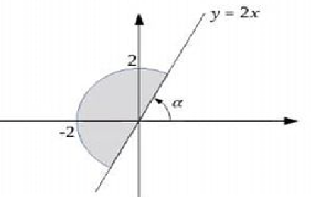
\includegraphics[scale=0.5]{img/rzutbrylyXY.png}
    \end{center}

    Zaznaczony na rysunku kąt $\alpha$ ma miarę $\arctan 2$.

    Współrzędne biegunowe centralne dają zatem:
    \[ 0 \leq r \leq 2, \quad \arctan 2 \leq \varphi \leq \arctan 2 + \pi \]

    Dostajemy
    \[ |U| = \iint\limits_D \left( \frac{1}{\left( 5 + \sqrt{x^2 + y^2}\right)^2} - 0 \right) \, dxdy = 
    \int\limits_{\arctan 2}^{\arctan 2 + \pi} d\varphi \int\limits_{0}^{2} r \, dr \cdot \frac{1}{(5 + r)^2} = \]
    \[ \pi \int\limits_{0}^{2} \frac{r}{(5+r)^2} \, dr = \pi \int\limits_{0}^{2} \frac{r + 5 - 5}{(5 + r)^2} \, dr = 
    \pi \int\limits_{0}^{2} \frac{1}{(5+r)} - \frac{5}{(5+r)^2} \, dr = \] 
    \[ \pi \left[ \ln |r + 5| + \frac{5}{r + 5} \right]_{0}^{2} = \pi \left( \ln 7 + \frac{5}{7} - \ln 5 - 1 \right) \]
\end{przyklad}

\begin{tw}{Definicja}
    Pole powierzchni płata krzywoliniowego
    \[ z = f(x,y), \quad (x,y) \in D \]

    Wzór jest analogiczny do długości krzywej \ $ y = f(x), \ a \leq x \leq b $ \ (AM1)
    \[ \text{Pole} = |\sum| = \iint\limits_D \sqrt{1 + f_x^2 + f_y^2} \, dxdy \]
\end{tw}

\begin{przyklad}
    Powierzchnia boczna stożka o promieniu podstawy $r$ i wysokości $h$.

    Sami ustawiamy stożek w układzie współrzędnych.

    Najłatwiejsze rozwiązania wychodzą, gdy wierzchołek będzie w początku układu współrzędnych, a oś symetrii stożka pokryje się z dodatnią częścią osi $Z$.

    Wtedy powierzchnia boczna będzie dana równaniem
    \[ z = f(x,y) = \frac{h}{r} \sqrt{x^2 + y^2} \]

    Zatem
    \[ f_x = \frac{h}{r} \cdot \frac{1}{2 \sqrt{x^2 + y^2}} \cdot 2x = \frac{h}{r} \cdot \frac{x}{\sqrt{x^2 + y^2}} \quad \text{oraz} \quad f_y = \frac{h}{r} \cdot \frac{y}{\sqrt{x^2 + y^2}} \]

    To daje
    \[ \sqrt{1 + f_x^2 + f_y^2} = \sqrt{1 + \frac{h^2}{r^2} \cdot \frac{x^2}{x^2 + y^2} + \frac{h^2}{r^2} \cdot \frac{y^2}{x^2 + y^2}} = \]
    \[ \sqrt{1 + \frac{h^2}{r^2}} = \frac{\sqrt{r^2 + h^2}}{r} = \frac{t}{r}, \quad \text{gdzie} \quad t = \sqrt{r^2 + h^2} \]

    Rzutem tej powierzchni na płaszczyznę jest $D$ -- koło o środku w (0,0) i promieniu $r$.

    Pole tej powierzchni wynosi zatem 
    \[ |\sum| = \iint\limits_D = \frac{l}{r} \, dxdy = \frac{l}{r} \iint\limits_D 1 \, dxdy = \frac{l}{r}|D| = \frac{l}{r} \cdot \pi r^2 = \pi r l \]
\end{przyklad}